%% Term Paper for EEET2493_labreport_template.tex
%% V1.0
%% 2020/04/17
%% This is the template for a Term Paper following an IEEE paper. Modified by Krishna Tulsyan after Francisco Tovar after Michael Sheel original document.

%%*************************************************************************
%% Legal Notice:
%% This code is offered as-is without any warranty either expressed or
%% implied; without even the implied warranty of MERCHANTABILITY or
%% FITNESS FOR A PARTICULAR PURPOSE! 
%% User assumes all risk.
%% In no event shall the IEEE or any contributor to this code be liable for
%% any damages or losses, including, but not limited to, incidental,
%% consequential, or any other damages, resulting from the use or misuse
%% of any information contained here.
%%
%% All comments are the opinions of their respective authors and are not
%% necessarily endorsed by the IEEE.
%%
%% This work is distributed under the LaTeX Project Public License (LPPL)
%% ( http://www.latex-project.org/ ) version 1.3, and may be freely used,
%% distributed and modified. A copy of the LPPL, version 1.3, is included
%% in the base LaTeX documentation of all distributions of LaTeX released
%% 2003/12/01 or later.
%% Retain all contribution notices and credits.
%% ** Modified files should be clearly indicated as such, including  **
%% ** renaming them and changing author support contact information. **
%%*************************************************************************

\documentclass[journal]{IEEEtran}

% *** CITATION PACKAGES ***
\usepackage[style=ieee]{biblatex} 
\bibliography{example.bib}    

% *** MATH PACKAGES ***
\usepackage{amsmath}

% *** BLINDTEXT PACKAGE ***
\usepackage{blindtext}

% *** PDF, URL AND HYPERLINK PACKAGES ***
\usepackage{url}
% correct bad hyphenation here
\usepackage{graphicx}  %needed to include png, eps figures
\usepackage{float}  % used to fix location of images i.e.\begin{figure}[H]

\begin{document}

% paper title
\title{Optimization Methods Term Paper}

% author names 
\author{Student name and roll no}% <-this % stops a space
        

% make the title area
\maketitle

% As a general rule, do not put math, special symbols or citations
% in the abstract or keywords.

\section{Introduction }
Include a title and one or two paragraphs describing what you plan to do and what your topic is all about. Be specific if you can. Include  one good reference you plan to used. This is an example of how to include a citation \cite{williams1989style}.  \\.

\textbf{The Sections included in this document are only for reference. Please use your own discretion to add/remove/modify the sections accordingly}.

\section {Background}
Give a background on your topic. Include references.

\blindtext
\blindtext
\blindtext

\section{Details}
\textbf{Discuss and describe the details of your specific topic. be thorough in your description and include references or figures/images when needed. One example of a figure is given below.}

You can refer to a Figure ~\ref{fig:man_with_camera} using this method.

\begin{figure}%[tbhp]
\centering
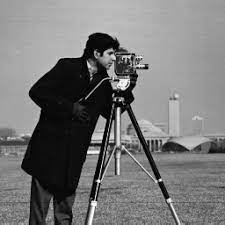
\includegraphics[width=.6\linewidth]{Figures/Figure_1}
\caption{Famous Placeholder image of a man shooting with camera}
\label{fig:man_with_camera}
\end{figure}

\blindtext
\blindtext

\section{Summary}
Summary of your paper.

\blindtext

\appendix
Optional.

\blindtext



\printbibliography

% that's all folks
\end{document}


